\documentclass[a4paper,10pt]{article}

\usepackage[spanish]{babel}
\usepackage[utf8]{inputenx}
\usepackage{booktabs}
\usepackage{multirow}
\usepackage{amssymb}
\usepackage{graphicx}
\usepackage{listings}
\usepackage{verbatim}
\newcommand{\here}{\checkmark}

\newenvironment{code}{\footnotesize\verbatim}{\endverbatim\normalsize}
\DeclareUnicodeCharacter{03BB}{$\lambda$}
\DeclareUnicodeCharacter{2192}{$\rightarrow$}

\title{Implementación de Lenguajes: Attribute Grammars}
\author{Alejandro Gadea \and Emmanuel Gunther}

\begin{document}
\maketitle
\lstset{ language=Haskell
       , literate={λ}{{$\lambda$}}1{→}{{$\rightarrow$}}1
	   }

\section{Sintaxis y semántica de Lenguajes}

\subsection{El problema RepMin}

El problema ``Rep Min'' es un ejemplo famoso del poder de la evaluación Lazy e inspira la construcción
de la manera de definir semántica que explotan las Attribute Grammars.

Consideremos el tipo de dato de los árboles binarios, con números enteros en las hojas. El problema
consiste en reemplazar cada valor de las hojas del árbol por el valor mínimo:

\begin{center}
 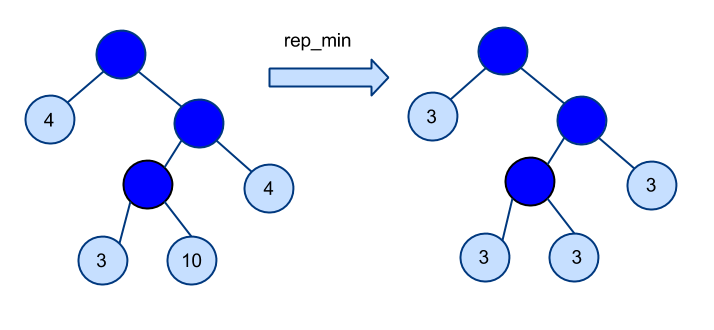
\includegraphics[height=4cm]{./repmin.png}
\end{center}

Podríamos definir un tipo de dato en Haskell para representar un árbol binario
de la siguiente manera:

\begin{lstlisting}
 data Tree =   Leaf Int 
	     | Bin (Tree,Tree)
\end{lstlisting}

Un árbol puede construirse a partir de un entero (una hoja) o a partir de otros
dos subárboles. Es decir, podemos construir un elemento de $Tree$ a partir
de un elemento de la unión disjunta $Int \sqcup (Tree\,\times\,Tree)$.
A esta unión disjunta la podemos definir en Haskell para cualquier tipo $a$:

\begin{lstlisting}
 type FTree a = Either Int (a,a)
\end{lstlisting}

\noindent y entonces podemos obtener cualquier elemento de $\mathbf{Tree}$ a partir de algún elemento de
$\mathbf{FTree\,Tree}$.

Al tipo de esta función que consiste en obtener un elemento de tipo $a$ a partir de uno de tipo
$\mathbf{FTree}\,a$ lo definimos explícitamente:

\begin{lstlisting}
 type FTreeAlgebra a = FTree a -> a
\end{lstlisting}



Si queremos definir entonces una semántica para los árboles binarios en un conjunto
semántico $B$ podemos definir una $\mathbf{FTreeAlgebra}\;B$. Para ello tenemos que dar
una regla para el caso en que partimos de un entero y otra regla para el caso en el que 
partimos de un par en $B\;\times\;B$.

La representación sintáctica de los árboles binarios con el tipo $Tree$ podría verse como una
semántica trivial y la podemos definir de la siguiente manera:

\begin{lstlisting}
  init_algebra :: FTreeAlgebra Tree
  init_algebra = either Leaf Bin
\end{lstlisting}

Si pensamos en términos de categorías, podemos ver a $FTree$ como un funtor que transforma
un objeto $A$ en un objeto $Int \sqcup (A\,x\,A)$ y entonces una $FTree-algebra$ será un morfismo
$\alpha\,:\,FTree\;A\;\rightarrow\;A$. Si $\alpha$ es la FTree-álgebra inicial entonces para cualquier otra
FTree-álgebra $\beta\,:\,FTree\;B\;\rightarrow\;B$ debe existir un único morfismo entre $\alpha$ y $\beta$, 
es decir, una única $f$ tal que el siguiente diagrama conmuta:

\begin{center}
 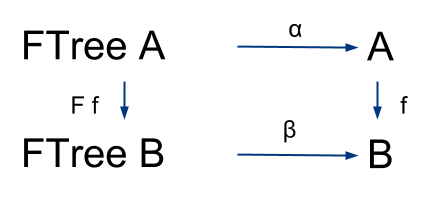
\includegraphics[height=3cm]{./Falgebras.png}
\end{center}

Si queremos entonces dar semántica a los árboles binarios debemos encontrar el único morfismo
entre $init\_algebra$ (el FTree-álgebra inicial) y otra FTree-álgebra. A este morfismo
se lo llama \textbf{catamorfismo}:

\begin{lstlisting}
  cataTree :: FTreeAlgebra b -> Tree -> b
  cataTree beta (Leaf i)    = beta (Left i)
  cataTree beta (Bin (t1,t2)) = beta (Right (cataTree beta t1,
					     cataTree beta t2))
\end{lstlisting}


Volviendo al problema que queremos resolver, a partir de un árbol queremos obtener
otro en el cual los valores de las hojas están reemplazados por el mínimo.

Una primera solución consiste en primero obtener el mínimo del árbol y luego reemplazar
por ese valor encontrado todas los valores de las hojas. Esto implica realizar dos 
recorridas al árbol inicial.

Para obtener el mínimo definimos una FTree-álgebra y definimos una función
que dado un entero $n$ construye la FTree-álgebra para reemplazar
los valores de las hojas por $n$:

\begin{lstlisting}
  min_alg :: FTreeAlgebra Int
  min_alg = either id (uncurry min)

  rep_min_alg :: Int -> FTreeAlgebra Tree
  rep_min_alg n = either (const $ Leaf n) Bin
\end{lstlisting}

Encontramos el resultado entonces llamando a la función $cataTree$
dos veces:

\begin{lstlisting}
  replace_min :: Tree -> Tree
  replace_min t = let n = cataTree min_alg t in
		      cataTree (rep_min_alg n) t
\end{lstlisting}

Observemos que en la función $rep\_min\_alg$ obtenemos el álgebra a partir de un entero.
En lugar de realizar esto, podríamos definir un álgebra que nos permita calcular una función
que dado un entero construye el árbol consistente en reemplazar todos los valores
por ese entero:

\begin{lstlisting}
  rep_min_alg' :: FTreeAlgebra (Int -> Tree)
  rep_min_alg' = either (const Leaf) 
                        (\(lfun,rfun) -> \m -> 
			    Bin (lfun m,rfun m))
\end{lstlisting}

\noindent y entonces el resultado a nuestro problema lo podemos obtener así:

\begin{lstlisting}
  replace_min' :: Tree -> Tree
  replace_min' t = (cataTree rep_min_alg' t) (cataTree min_alg t) 
\end{lstlisting}

Podemos ver en esta última definición que las dos llamadas a la función $cataTree$ son independientes
entre sí por lo que podríamos calcular una sola FTree-álgebra que obtenga ambos resultados
simultáneamente. Con $min\_alg$ calculamos el mínimo y con $rep\_min\_alg'$ la función para construir
el árbol, por lo cual si pudiéramos realizar el producto de esas dos FTree-álgebras obtendríamos ambos
resultados:

\begin{lstlisting}
  infix 9 `x`

  x :: FTreeAlgebra a -> FTreeAlgebra b -> FTreeAlgebra (a,b)
  fa `x` fb = either  (\i -> (fa $ Left i,fb $ Left i))
		      (\((a,b),(a',b')) -> 
			(fa $ Right (a,a'),fb $ Right (b,b')))
			  

  rep_min_alg'' :: FTreeAlgebra (Int,Int -> Tree)
  rep_min_alg'' = min_alg `x` rep_min_alg'
  
\end{lstlisting}

  Ahora entonces podemos obtener el resultado al problema realizando una sola llamada
  a $cataTree$:
  
\begin{lstlisting}
 replace_min'' :: Tree -> Tree
 replace_min'' t = r m
    where (m, r) = cataTree rep_min_alg'' t
\end{lstlisting}

  Para realizar nuestra última mejora, consideremos la siguiente función que dados dos
  tipos isomorfos $a$ y $b$, y una $FTreeAlgebra\;a$, obtiene una $FTreeAlgebra\;b$:

  \begin{lstlisting}
   getIsoAlg :: (a -> b) -> (b -> a) -> FTreeAlgebra a -> FTreeAlgebra b
   getIsoAlg fab fba fa = either (fab . fa . Left)
                                 (fab . fa . Right . (fba *** fba))
  \end{lstlisting}
  
  En nuestro problema tenemos una FTree-álgebra de tipo 
  
  \begin{lstlisting}
   (Int,Int -> Tree)
  \end{lstlisting}
  
  Y para nuestro problema, la podemos considerar equivalente al tipo (explicar esto)
  
  \begin{lstlisting}
   Int -> (Int,Tree)
  \end{lstlisting} 
  
  Necesitaríamos dos funciones para intercambiar estos tipos tal que sean una inversa de la otra:
  
  \begin{lstlisting}
   f1 :: (Int,Int -> Tree) -> (Int -> (Int,Tree))
   
   f2 :: (Int -> (Int,Tree)) -> (Int,Int -> Tree)
  \end{lstlisting}

  La primera de estas la podemos construir fácilmente, pero para la segunda encontramos un problema
  ya que para obtener el primer elemento del par no sabríamos qué valor pasarle a la función argumento:
    
  \begin{lstlisting}
   f1 :: (Int,Int -> Tree) -> (Int -> (Int,Tree))
   f1 (i,f) = const i &&& f

   f2 :: (Int -> (Int,Tree)) -> (Int,Int -> Tree)
   f2 f = (??? , snd . f)
  \end{lstlisting}

  hay que seguir...
 
  
  

% de los árboles binarias con el tipo $Tree$ constituyen el álgebra inicial, que consiste en
% aplicar la función $Leaf$ si el elemento es un entero, y la función $Bin$ si 



\subsection{Repmin con Attribute Grammars}

  En la sección previa vimos cómo resolver el problema Repmin de una manera más eficiente realizando
  una sola recorrida al árbol, gracias a la evaluación Lazy de Haskell. Para ello obteníamos
  una tupla en donde el primer elemento era el mínimo de árbol y el segundo elemento una función
  que dado un entero construye el árbol resultante de reemplazar los valores en las hojas por ese entero.
  
  Observemos que podríamos realizar el mismo procedimiento para cualquier tipo de dato recursivo, donde
  la gramática no necesariamente conste de dos producciones. Podríamos definir el funtor $F$ 
  y el catamorfismo correspondiente. Luego para calcular una semántica solo necesitamos tener una regla
  para cada producción de la gramática.
  
  Con \textbf{Attribute Grammars} tenemos una notación sencilla para definir semántica definiendo la sintaxis
  de un tipo de datos y luego dando reglas para cada producción de la gramática. Un preprocesador
  convierte esta notación en código Haskell que es equivalente al que obtuvimos en la sección previa.
  
  El problema RepMin podemos resolverlo de esta manera con Attribute Grammars:
  
  \begin{lstlisting}
   data Tree
      | Leaf      Int
      | Bin lt :: Tree
	    rt :: Tree

  deriving Tree : Show
	  
  attr Tree
      inh minval :: Int
      syn m      :: Int
      syn res    :: Tree
      
  sem Tree
      | Leaf lhs.m   = @int
		.res = Leaf @lhs.minval
      | Bin  lhs.m   = @lt.m `min` @rt.m
		.res = Bin @lt.res @rt.res
		
  data Root
      | Root Tree
      
      
  attr Root
      syn res :: Tree
      
  sem Root
      | Root tree.minval = @tree.m
  \end{lstlisting}

  La definición de la gramática es similar a lo que definimos en Haskell, solo que ponemos nombres
  a cada parámetro en cada producción. Para calcular semántica definimos atributos, los sintetizados ($syn$)
  son aquellos que para calcular el valor en un nodo necesitamos saber el valor en los hijos, y los heredados ($inh$)
  son pasados a través del árbol de arriba hacia abajo.
  
  En nuestro ejemplo necesitamos el valor mínimo del árbol para poder calcular el resultado a repmin y entonces definimos
  un atributo heredado $minval$. El atributo sintetizado $m$ calcula el mínimo del árbol y con ese valor se inicializa
  $minval$ que es utilizado luego para calcular el $res$.
  
  En el código mostrado se utilizan muchas abreviaciones que permiten escribir código más corto. Por ejemplo, si una regla
  de producción en la gramática tiene un solo argumento, puede obviarse definir el nombre explícitamente y se genera uno
  consistente del nombre del tipo de dato con la primera letra en minúscula. Si un atributo heredado no cambia el valor
  al pasar al nodo hijo, entonces no es necesario definir esa regla trivial.
  
  El código generado utilizando \textbf{Attribute Grammars} calcula los valores de los atributos realizando el procedimiento
  que mostramos en la sección previa. El tipo del álgebra resultante será una función donde los parámetros son los atributos
  heredados y el resultado será una tupla donde cada elemento de la tupla es un atributo sintetizado.
  
  
%   En general podemos tener muchos problemas donde necesitemos calcular algunos valores en una estructura de datos
%   que luego tengan que ser utilizados para calcular otros valores, con estructuras recursivas más complicadas
%   que los árboles binarios. Realizar todo el proceso que mostramos puede ser tedioso y propicio para cometer
%   errores
  
  


\section{El cálculo Lambda}

En la sección pasada vimos como podemos definirnos una función de manera general,
que llamábamos catamorfismo, y como esta definición nos induce la introducción
de una sintaxis especial con la idea de que solo haga falta implementar lo relativo
al problema. 

A continuación vamos a implementar un inferidor de tipos para el cálculo lambda 
simplemente tipado, así también como su parser y pretty printing.

\subsection{Sintaxis: Parser y Pretty Printing}

\subsubsection{Sintaxis}

$Var$ $::=$ Conjunto numerable. En general serán $a$, $b$, $c$, $x$, $y$, $z$, etc.


\begin{lstlisting}
Term ::= Var
       | λ Var . Term
       | Term Term
\end{lstlisting}


\subsubsection{Parser}

La implementación de un parser para la sintaxis del calculo lambda es mas bien
simple y directa, aun incluso agregando la restricción de que solo permitimos parsear
términos cerrados, es decir términos en los cuales no aparecen variables libres.
Sin embargo, supongamos tenemos el siguiente termino a parsear,\\

$\lambda a . s$\\

claramente ``s'' es libre, pero no estaría mal suponer que en realidad ese termino
bien podría haber sido\\

$\lambda a . a$\\

es decir, se cometió un error al escribir el termino. Por lo tanto, un parser
algo mas interesante podría ser uno tal que detecte este tipo de errores, los
corrija e informe sobre tal decisión.\\

Ahora bien, para la implementación del parser utilizamos la librería ``uu-parsinglib''
la cual provee exactamente una corrección de errores. Por ejemplo, siendo ``pa''
el parser de la letra ``a'', al intentar parsear ``b'' obtenemos "a" donde lo que
sucedió fue el reemplazo de ``b'' por ``a'':\\

\begin{code}
 >>> run pa  "b"
     Result: "a"
     Correcting steps: 
       Deleted   'b' at position LineColPos 0 0 0 expecting 'a'
       Inserted  'a' at position LineColPos 0 1 1 expecting 'a'
\end{code}

Algo a destacar es que la corrección de errores que pretendemos para nuestro
parser de términos es casi gratuita. En un resumen preliminar, para parsear el
cuerpo de una abstracción solamente tenemos que tener una lista de las variables
introducidas hasta ese momento y generar parser's para cada nombre de variable
en esa lista.\\

Antes de presentar los parser relativos a cada construcción de la gramática,
definamos algunos parsers generales que nos van a ser de utilidad.

\begin{lstlisting}
parseTermSym :: Parser String -> [String] -> Parser String
\end{lstlisting}
Generamos un parser a partir de un parser por default y una lista de strings.

\begin{lstlisting}
parseXSym :: Parser String
\end{lstlisting} con X $\in$ {Lam,Dot,App}\\

Parsers para los símbolos $\lambda$, $.$ y $@$. Donde además podemos parsear 
``\textbackslash \textbackslash'' en lugar de $\lambda$ y $->$ o $\rightarrow$
en lugar de ``$.$'' .

\begin{lstlisting}
parseVar :: Parser Var
\end{lstlisting} Parser de variables.\\

Ahora sí, dada la lista de variables a parsear, digamos $vars$, parsear un
identificador de variable será generar parsers para cada variable de la lista
y fallar parser default:

\begin{lstlisting}
parseId :: [Var] -> Parser Term
parseId vars = Id <$> parseTermSym pFail vars
\end{lstlisting}

Lo interesante a destacar es que en la generación de parsers para las variables,
esta contenida la acción de corregir una ocurrencia de variable libre.\\

Para el caso de la abstracción, dejando de lado el parseo de los símbolos respectivos,
vamos a parsear una variable y se podría decir que la necesitamos para dos cosas;
(1) el constructor de la abstracción, (2) la lista de variables posibles a parsear.
Esto genera un problema, ya que al parsear la variable esta queda encapsulada 
dentro de la computación ``Parser Var'', por (2) podemos pensar que el parser encargado
de parsear el cuerpo de la abstracción tiene el siguiente tipo $Var -> Parser Term$,
ya que toma la variable la añade a la lista de variables y parsea el termino.
Si ahora prestamos atención necesitamos una función que convine, parsear la variable con
parsear un termino agregando esa variable, es decir una función con tipo:

\begin{lstlisting}
Parser Var -> (Var -> Parser Term) -> Parser Term
\end{lstlisting}

pero este es justamente el tipo del bind ($>>=$), $m \ a \rightarrow (a \rightarrow m \ b) \rightarrow m \ b$. Esto
nos obliga a usar mónadas entonces para lo cual necesitamos la función addLength.
No estamos seguros si existe una manera de resolver esto sin usar mónadas, con el
fin de evitar el uso de addLength. La definición final entonces queda,

\begin{lstlisting}
parseAbs :: [Var] -> Parser Term
parseAbs vars = 
       addLength 1 $
       join $ uncurry (<$>) 
           <$> 
       (Abs &&& parseTerm . (:vars))
       	   <$ 
       parseLamSym <*> parseVar <* parseDotSym
\end{lstlisting}

Concluyendo, para el caso de la aplicación será parsear identificadores de variable
o abstracciones separadas por ``$@$'', para esto nos definimos un parser particular
para estos parsers,

\begin{lstlisting}
parseTerm' :: [Var] -> Parser Term
parseTerm' vars =  parseId vars
               <|> parseAbs vars
               <|> pParens (parseTerm vars)\\

parseApp :: [Var] -> Parser Term
parseApp vars = (App <$ parseAppSym) `pChainl` (parseTerm' vars)
\end{lstlisting}

luego, parsear un termino será simplemente el parser definido para la applicación,\\

\begin{lstlisting}
parseTerm :: [Var] -> Parser Term
parseTerm vars = parseApp vars
\end{lstlisting}

En conclusión, tenemos un parser para la gramática anterior que además corrige 
algunos errores, como el mencionado al comienzo. Algo importante a mencionar es
que la corrección de errores puede tener algún que otro comportamiento no deseado
como consecuencia de una implementación "simplista" en términos del uso del 
poder de corrección de la librería. Un ejemplo de esto podría ser,

\begin{verbatim}
*Parser> parserTerm "\\a -> b@a"
(λ a → a
, [-- Deleted   'b' at position LineColPos 0 6 6 expecting Whitespace
  ,-- Deleted   '@' at position LineColPos 0 7 7 expecting "a"
  ]
)
\end{verbatim}

donde muy probablemente la corrección deseada hubiera sido simplemente reemplazar
b por a, y generar el termino $\lambda$ a $\rightarrow$ a@a.

\subsubsection{Pretty Printing}

La implementación del pretty printing nos interesa como un primer pequeño paso
hacía de definición de una función semántica para el tipo de dato $Term$ utilizando
AG. En resumen, la semántica que estamos pensando trasformaría un $Term$, es decir
un termino del calculo lambda, en su representación en $String$.\\

A pesar de tener pocos constructores un termino del calculo lambda puede ser 
complejo de leer y una ``organización'' de los subterminos a la hora de escribirlo
puede ayudar mucho a la interpretación. Por ejemplo, el termino
$(\lambda x \rightarrow x@x)@(\lambda x \rightarrow x@x)$ no genera problema pero en
cambio si tenemos, 
$(\lambda x \rightarrow
	\lambda y \rightarrow
		\lambda f \rightarrow f @ (x @ (\lambda w \rightarrow f @ w)) @ (y @ f @ x))$
$@$
$(\lambda x \rightarrow 
	\lambda y \rightarrow \lambda f \rightarrow 
	\lambda g \rightarrow \lambda h \rightarrow h @ (f @ x) @ (g @ y))$
$@$ $\lambda x \rightarrow \lambda f \rightarrow 
		\lambda g \rightarrow f @ g @ (x @ g)$
puede ser difícil de leer. Por lo tanto una buena presentación del termino puede
ayudar mucho. La utilización de la librería ``uulib'', en particular de ``UU.PPrint'', 
nos brinda una manera de implementar un pretty printing de manera simple.\\

Como vimos para el caso de Repmin, deberíamos definir atributos y dar reglas para
cada constructor, esta vez para $Term$, que expresen como trasformar cada uno en
su representación en $String$.\\

Queremos un atributo sintetizado, que llamamos ``pprint'', que sea el resultado
de transformar un $Term$ a un $String$ y un atributo heredado que necesitamos para
saber cuando encerrar un termino entre paréntesis o no.

\begin{lstlisting}
attr Term 
    syn pprint :: {Doc}
    inh paren  :: {ParenInfo}
\end{lstlisting}

Por otro lado la semántica estará definida como,

\begin{lstlisting}    
sem Term
\end{lstlisting}
Para el identificador de variable será simplemente imprimir su nombre de variable
recordando que estos estaban ya representados por $String$'s
\begin{lstlisting}    
    | Id  lhs.pprint  = text @ident
\end{lstlisting}

En el caso de la aplicación, comencemos explicando que imprimir una aplicación será
simplemente imprimir su lado izquierdo (lt) y su lado derecho (rt) pero teniendo
algunas consideraciones; En cuando a los paréntesis, la aplicación asocia a izquierda
por lo tanto si tenemos, por ejemplo, la aplicación de $x@y$ y $z@w$ vamos a necesitar
colocar paréntesis solamente en el lado derecho ($rt.paren = Paren$) para imprimir la
correcta aplicación $x@y@(z@w)$. Pero además, hay un caso particular donde el lado
izquierdo de la aplicación lleva paréntesis y ese es cuando en ese lado hay una
abstracción, por ejemplo aplicando $\lambda x \rightarrow x$ y $z@w$. Por esto solamente
colocamos paréntesis en un lado izquierdo si este es una abstracción ($lt.paren = ParenAbs$).
Notar que sin los paréntesis las aplicaciones de los ejemplos quedarían $x@y@(z@w)$ y 
$\lambda x \rightarrow x@z@w$ las cuales no son representaciones de los términos originales.\\

Ahora bien, dejando de lado los paréntesis, para imprimir una aplicación la idea será
intentar que tanto el lado izquierdo como el derecho estén en el mismo nivel y en caso
de que esto no sea posible obtener lo siguiente,

\begin{center}
$lt$\\
$@$\\
$rt$
\end{center}

es decir, separar los subterminos en dos niveles intercalando el operador de aplicación.
Con la posibilidad de ubicar el lado derecho en el mismo nivel del operador.

\begin{lstlisting}    
    | App lhs.pprint  = (putParen @lhs.paren) 
                (group $ @lt.pprint <> line <> 
                  (group $ text "@" <> line <> @rt.pprint)
                )
          rt.paren    = Paren
          lt.paren    = ParenAbs
\end{lstlisting}    

Para terminar, nos falta definir la semántica para el caso del constructor de la
abstracción. Para este caso la idea será si podemos escribir toda la abstracción
en el mismo nivel lo hacemos, de no ser posible vamos a imprimir el cuerpo ($term$)
en otro nivel con un cierto identado (3 caracteres) para ayudar a identificar el
cuerpo de la abstracción cuando esta aplicada con un termino. Por otro lado, en el
cuerpo nunca hace falta poner paréntesis ($term.paren = NoParen$).

\begin{lstlisting}
    | Abs lhs.pprint  = (putAbsParen @lhs.paren)
                (text "λ " <> text @var <> text " →" <> 
                    group (nest 3 $ line <> @term.pprint)
                )
          term.paren  = NoParen
\end{lstlisting}

Imprimiendo el ejemplo del comienzo podemos notar que es mucho mas sencillo de
leer. En particular contiene muchas de las variantes de impresión posibles que
implementa la semántica que dimos.

\begin{verbatim}
*Main> App (App t2 t3) t1
(λ x →
   λ y →
      λ f → f @ (x @ (λ w → f @ w)) @ (y @ f @ x))
@
(λ x →
   λ y → λ f → λ g → λ h → h @ (f @ x) @ (g @ y))
@ (λ x → λ f → λ g → f @ g @ (x @ g))
\end{verbatim}

\subsection{Inferidor de tipos}
 
\end{document}
